%Argonne 2023 May 18 Argonne Talk
\documentclass[10pt,compress,xcolor={usenames,dvipsnames},aspectratio=169]{beamer}
%\usepackage[T1]{fontenc}
%\usepackage{tgadventor} %Font found at https://tug.org/FontCatalogue/
%\usepackage{newpxtext}
\usepackage{newtxtext}
%\usepackage[light]{antpolt}
\usepackage[T1]{fontenc}
\usepackage{datetime2}
%\usepackage[euler-digits,euler-hat-accent]{eulervm}


\usepackage{amsmath,
	amssymb,
	datetime,
	mathtools,
	bbm,
	%mathabx,
	array,
	booktabs,
	xspace,
	multirow,
	calc,
	colortbl,
	siunitx,
	centernot,
 	graphicx}
\usepackage[usenames]{xcolor}
\usepackage[giveninits=false,
backend=biber,
style=nature,
style=authoryear-comp,
maxcitenames=4,
mincitenames=2]{biblatex}
\addbibresource{FJHown23.bib}
\addbibresource{FJH23.bib}
\usepackage{media9}
\usepackage[autolinebreaks]{mcode}
\usepackage[tikz]{mdframed}
\graphicspath{{figures/}}


\usetheme{FJHSlimNoFoot169}
\setlength{\parskip}{2ex}
\setlength{\arraycolsep}{0.5ex}
\setbeamertemplate{itemize subitem}[triangle]
\setbeamerfont{footnote}{size=\scriptsize}

\DeclareMathOperator{\SOL}{SOL}
\DeclareMathOperator{\APP}{APP}
\DeclareMathOperator{\ERR}{ERR}
\DeclareMathOperator{\AVG}{AVG}
\DeclareMathOperator{\INT}{INT}
\DeclareMathOperator{\LIN}{LINEAR}
\DeclareMathOperator{\BAD}{BAD}
\DeclareMathOperator{\DISC}{DSC}
\DeclareMathOperator{\VAR}{VAR}
\DeclareMathOperator{\CONF}{CNF}
%\DeclareMathOperator{\opt}{opt}
\newcommand{\dataN}{\bigl(\hf(\vk_i)\bigr)_{i=1}^n}
\newcommand{\dataNj}{\bigl(\hf(\vk_i)\bigr)_{i=1}^{n_j}}
\newcommand{\dataNjd}{\bigl(\hf(\vk_i)\bigr)_{i=1}^{n_{j^\dagger}}}
\newcommand{\ERRN}{\ERR\bigl(\dataN,n\bigr)}
\newcommand{\otod}{\ensuremath{1\mkern-4mu : \mkern-2mu d}}


\iffalse
Title:  Faster Monte Carlo via Low Discrepancy Sampling
Speaker:  Fred J. Hickernell, Illinois Institute of Technology

Abstract:  Estimating an expectation or integral is important in high energy physics, Bayesian inference, image rendering, quantitative finance, and uncertainty quantification.  Monte Carlo type methods are commonly used.  The numerical error can be expressed as a product of three quantities: one measuring the deficit in the sampling scheme, a second measuring the roughness of the function defining the expectation or integral, and a third representing the confounding between that function and the sampling deficit.  We explain how low discrepancy sampling, also known as the quasi-Monte Carlo method, can substantially improve the efficiency of these calculations.  We discuss how to improve efficiency via transformations of the integral.  Our data-driven error bounds advise the user when to stop simulating.  We illustrate low discrepancy sampling via our QMCPy software library (qmcpy.org).

Bio: Fred J. Hickernell is Professor of Applied Mathematics and Vice Provost for Research at Illinois Institute of Technology.  Although his father and brothers are physicists, Fred's physical intuition was lacking so he pursued a PhD in applied mathematics.  For the past three decades, Fred has explored how to improve the efficiency of Monte Carlo methods through low discrepancy sampling, also known as the quasi-Monte Carlo method.  Recently, he and his collaborators have developed data-driven error bounds for quasi-Monte Carlo methods and have been encouraging greater application of quasi-Monte Carlo methods through the QMCPy software library.

\fi

%\DeclareMathOperator{\app}{app}

\providecommand{\HickernellFJ}{H.\xspace}
\DeclareMathOperator{\RMS}{RMS}


\renewcommand{\OffTitleLength}{-12ex}
\setlength{\FJHThankYouMessageOffset}{-8ex}
\title{Speedy Simulations}
\author[]{Sou-Cheng Choi and Fred J. Hickernell}
\institute{Illinois Institute of Technology \\
    Dept Applied Math \quad
	Ctr Interdisc Scientific Comput \quad Office of Research\\
 \href{mailto:schoi32@iit.edu}{\url{schoi32@iit.edu}}
	\\
	\href{mailto:hickernell@iit.edu}{\url{hickernell@iit.edu}} \qquad
	\href{https://sites.google.com/iit.edu/fred-j-hickernell}{\url{sites.google.com/iit.edu/fred-j-hickernell}}}

\thanksnote{Looking forward to working with you this summer \\
Slides at  \href{https://speakerdeck.com/fjhickernell/argonne2023maytalk}%
{\nolinkurl{speakerdeck.com/fjhickernell/argonne2023maytalk}} \\
Jupyter notebook with computations and figures \href{https://github.com/QMCSoftware/QMCSoftware/blob/develop/demos/talk_paper_demos/Argonne_Talk_2022_May/Argonne_2023_Talk_Figures.ipynb}{\beamerbutton{here}}\quad Visit us at \href{https://qmcpy.org}{\nolinkurl{qmcpy.org}}}

\event{SURE Kickoff}
\date[]{ revised \today}

\input FJHDef.tex

	\newcommand{\scoop}[1]{\parbox{#1}{\includegraphics[width=#1]{IceCreamScoop.eps}}\xspace}
\newcommand{\smallscoop}{\scoop{1cm}}
\newcommand{\medscoop}{\scoop{1.8cm}}
\newcommand{\largescoop}{\scoop{3cm}}
\newcommand{\ICcone}[1]{\parbox{#1}{\includegraphics[width=#1,angle=270]{MediumWaffleCone.eps}}\xspace}
\newcommand{\medcone}{\ICcone{1.2cm}}
%\newcommand{\medcone}{\parbox{1.1cm}{\includegraphics[width=1.2cm,angle=270]{MediumWaffleCone.eps}}\xspace}
\newcommand{\largercone}{\parbox{2.2cm}{\vspace*{-0.2cm}\includegraphics[width=1cm,angle=270]{MediumWaffleCone.eps}}\xspace}
\newcommand{\hugecone}{\parbox{4cm}{\vspace*{-0.2cm}\includegraphics[width=1.8cm,angle=270]{MediumWaffleCone.eps}}\xspace}
\newcommand{\largecone}{\ICcone{1.8cm}}
\newcommand{\smallcone}{\parbox{1.1cm}{\includegraphics[width=0.5cm,angle=270]{MediumWaffleCone.eps}}\xspace}


\begin{document}
	\everymath{\displaystyle}

\frame{\titlepage}

%%%%%%%%%%%%%%%%%%%%%%%%%%%%%%%%%%%%%%%%%%
%%%%%%%%%%%%%%%%%%%%%%%%%%%%%%%%%%%%%%%%%%
\section{Why Quasi-Monte Carlo Is Faster}
%%%%%%%%%%%%%%%%%%%%%%%%%%%%%%%%%%%%%%%%%%
%%%%%%%%%%%%%%%%%%%%%%%%%%%%%%%%%%%%%%%%%%


\begin{frame}{Uncertainty in a Cantilevered Beam\footfullcite{ParSee22a}}
	\vspace{-4ex}
	\begin{tabular}{m{0.6\textwidth}m{0.4\textwidth}}
		\[
		\begin{aligned}
			u(x) & = g(\vZ, x) = \text{beam deflection} \\
			x &= \text{position} \\
			& = \text{solution of a differential equation boundary value problem} \\
			\vZ & \sim \cu[1,1.2]^3 \quad \text{defines uncertainty in Young's modulus}
                & = \text{the randomness in the problem}\\
			\mu(x) &= \text{expected or mean value of the beam deflection} \\
                    & = \Ex[g(\vZ,x)] = \int_{[0,1]^3}  g(\vz,x) \, \dif \vz \approx 
                    \underbrace{\frac 1n \sum_{i=1}^n g(\vZ_i,x)}_{\substack{\text{\alert{sample mean} or }\\ \text{\alert{Monte Carlo estimate}}}}
			\\
			& \mu(\text{end}) = 1037  \qquad \text{\alert{How?}}
		\end{aligned}
		\]
		&
		\centering
		\vspace{1.5ex}
		\includegraphics[width=0.35\textwidth]{BeamDrawing.png} \newline
	\end{tabular}


\end{frame}


\begin{frame}{Simple vs.\ Quasi-Monte Carlo for the Cantilevered Beam via QMCPy\footfullcite{QMCPy2020a}}
	\vspace{-16ex}
	\begin{tabular}{m{0.63\textwidth}m{0.35\textwidth}}
		\[
		\begin{aligned}
				g(\vZ, x) &= \text{beam deflection} \\
			\only<1>{\vZ & \sim \cu[1,1.2]^3 \quad \text{defines uncertainty} &
			x &= \text{position} \\}
			\mu(x) &= \Ex[g(\vZ, x)] \approx 
                    \underbrace{\frac 1n \sum_{i=1}^n g(\vZ_i,x)}_{\text{\alert{Monte Carlo estimate}}} &
			\mu(\text{end}) &= 1037
		\end{aligned}
		\]
  	\vspace{-11ex}\only<2>{\vspace{-8ex}}
	\includegraphics<1>[width=0.6\textwidth]{iidldbeam.eps}
	\includegraphics<2>[width=0.5\textwidth]{ldparallelbeam.eps}
		&
		\centering
		\includegraphics[width=0.33\textwidth]{cantileveredbeamwords.eps}
	\end{tabular}


\end{frame}


\begin{frame}{Simple or Independent and Identically Distributed (IID) Monte Carlo}

\vspace{-10ex}
\includegraphics[width=\textwidth]{iidptsseq.eps}

Gaps and clusters, uneven

\end{frame}


\begin{frame}{Low Discrepancy Sampling aka  Quasi-Monte Carlo\footfullcite{Hic97a}}

	\vspace{-5ex}
	\hspace*{-2ex}
	\begin{tabular}{m{0.65\textwidth}m{0.35\textwidth}}
		\vspace{-4ex}
		\[
        \begin{aligned}
		    \MoveEqLeft{\overbrace{\int_{[0,1]^d} f(\vx) \, \dif \vx}^
            {\Ex[f(\vX)], \ \vX \sim \cu[0,1]^d} - \frac 1n \sum_{i=0}^n f(\vx_i)
			= \CONF(f,\{\vx\}_{i=1}^n) \, \DISC(\{\vx\}_{i=1}^n) \, \VAR(f)} \\
        \only<6>{ \MoveEqLeft{\CONF(f,\{\vx_i\}_{i=1}^n) = \frac{\int_{[0,1]^d} f(\vx) \, \dif \vx - \frac 1n \sum_{i=0}^n f(\vx_i)}{\DISC(\{\vx_i\}_{i=1}^n) \, \VAR(f)}   \quad \text{between } \pm1}}
         \only<2-5>{\MoveEqLeft{\DISC^2(\{\vx_i\}_{i=1}^n) = \left(\frac{13}{12}\right)^2} \\
         &
         - \frac 2n \sum_{i=1}^n \prod_{j=1}^d\left(1 + 0.5\abs{x_{ij} - 0.5} - 0.5(x_{ij}-0.5)^2\right) \\
         & + \frac{1}{n^2} \sum_{i,k=1}^n \left[ 1 + 0.5\abs{x_{ij} - 0.5} +
         0.5\abs{x_{kj} - 0.5} - 0.5\abs{x_{ij} - x_{kj}}\right]}
         \only<1>{\MoveEqLeft{\VAR^2(f)
          = \int_{[0,1]} \left[\frac{\partial f}{\partial x_1} (x_1, 0.5, \ldots, 0.5)\right]^2 \, \dif x_1 + \cdots }\\
         & + \int_{[0,1]^{2}} \left[\frac{\partial^2 f}{\partial x_1 \partial x_2} (x_1, x_2,0.5, \ldots, 0.5)\right]^2 \, \dif x_1 \, \dif x_2 + \cdots \\
         & + \int_{[0,1]^{d}} \left[\frac{\partial^d f}{\partial x_1 \cdots \partial x_d} (\vx)\right]^2 \, \dif \vx
         }
		\end{aligned}
        \]
		&
		\centering
		\only<1-2,6>{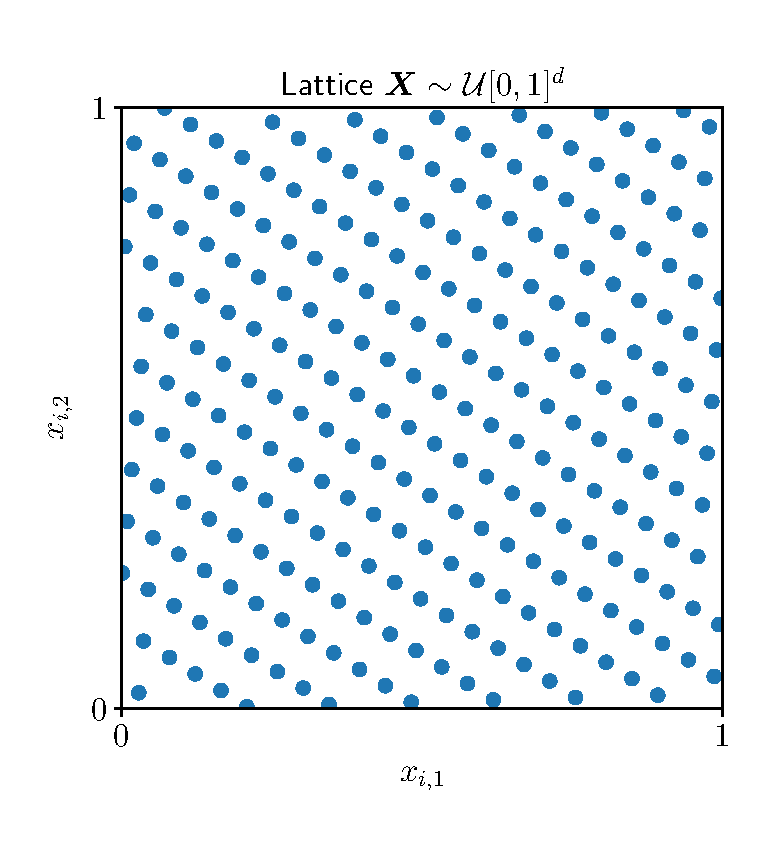
\includegraphics[width=0.35\textwidth]{latticeptssingle.eps}}
		\only<3>{\includegraphics[width=0.35\textwidth]{sobolptssingle.eps}}
		\only<4>{\includegraphics[width=0.35\textwidth]{haltonptssingle.eps}}
		\only<5>{\includegraphics[width=0.35\textwidth]{iidptssingle.eps}}
		\only<2-4,6>{\vspace{-4ex}
		\[\DISC(\{\vx_i\}_{i=1}^n) = \alert{\Order(n^{-1+\delta})}\]}
		\only<5>{\vspace{-4ex}
	\[\DISC(\{\vx_i\}_{i=1}^n) = \alert{\Order(n^{-1/2})}\]}
	\end{tabular}
	\vspace{-5ex}

        \only<1>{$\VAR$ is a semi-norm, more smoothness than $\std$, value generally unknown, reduced through transformations}%
        \only<2>{\vspace{-1ex} $\DISC$ is the norm of the error functional, value known with $\Order(dn^2)$ operations}

\end{frame}




\begin{frame}{Low Discrepancy Points Fill Space Better Than IID Points}
\vspace{-3.2ex}

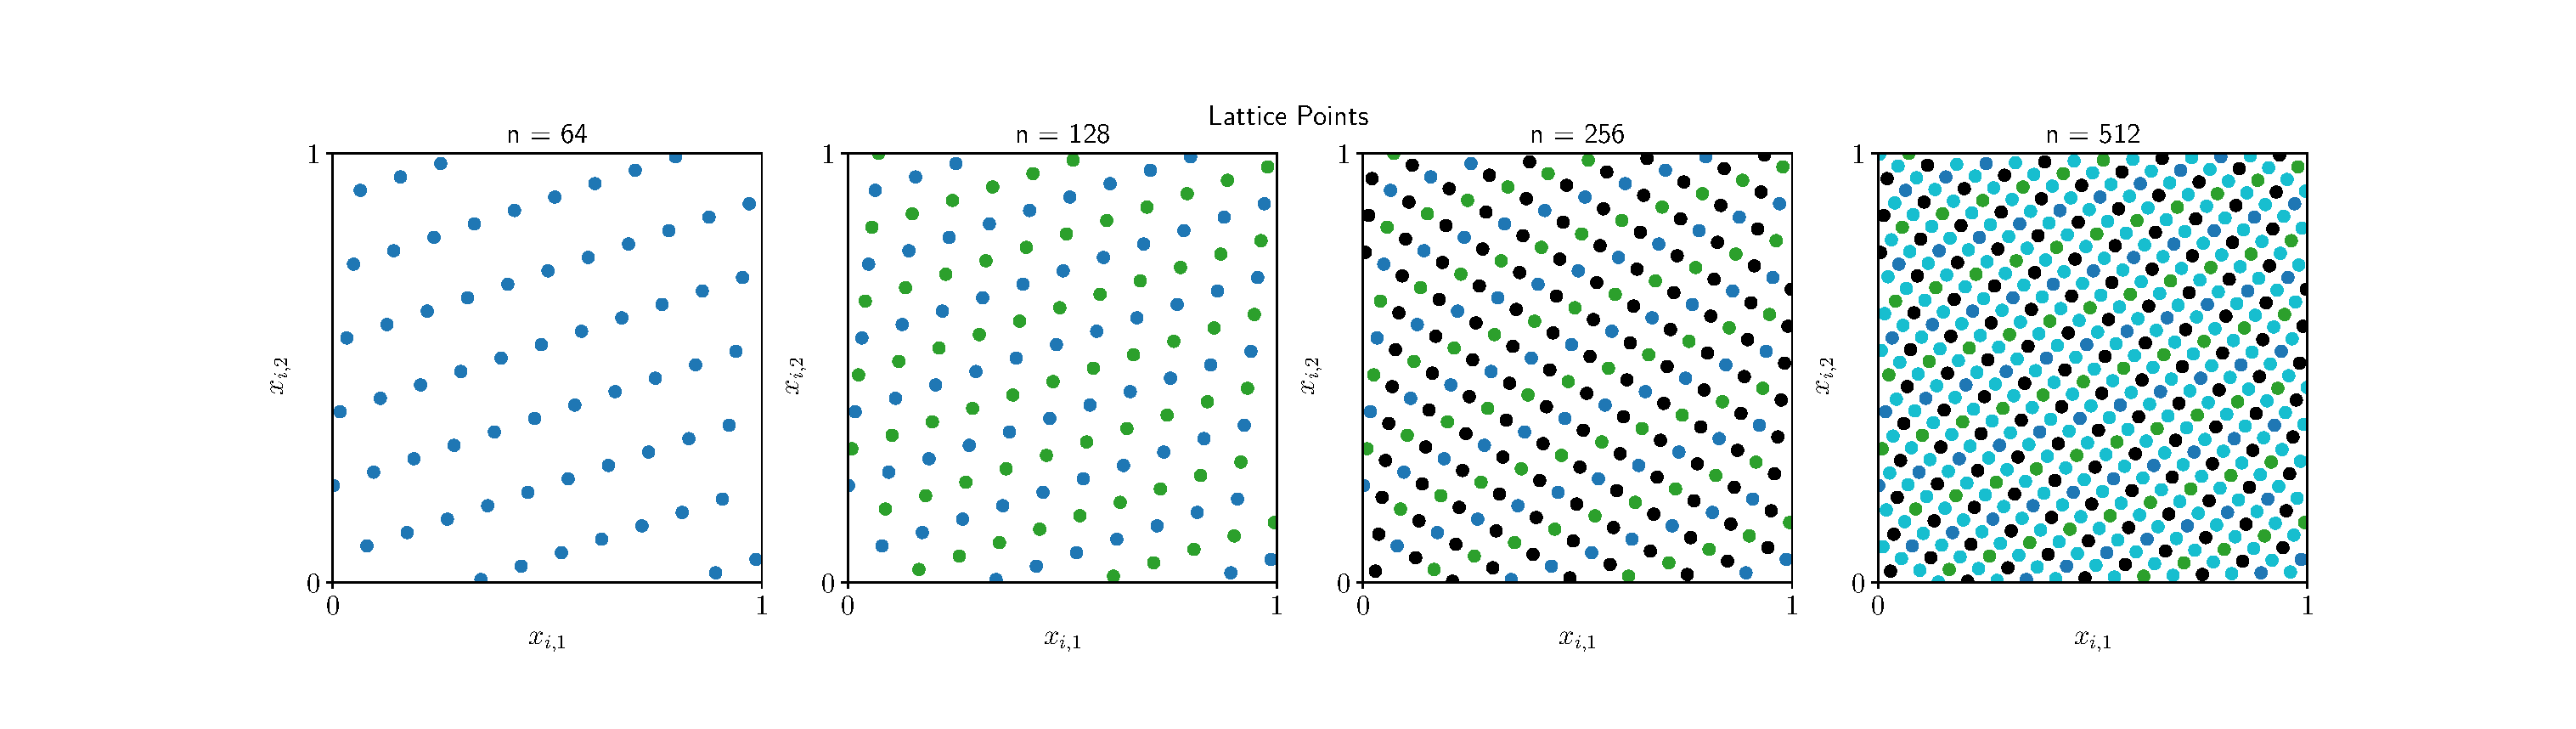
\includegraphics[width=\textwidth]{latticeptsseq.eps}

\vspace{-4.3ex}

\includegraphics[width=\textwidth]{sobolptsseq.eps}

\end{frame}

\begin{frame}{Low Discrepancy Points Look ``Good'' in All Coordinate Projections}
	\vspace{-3.2ex}

	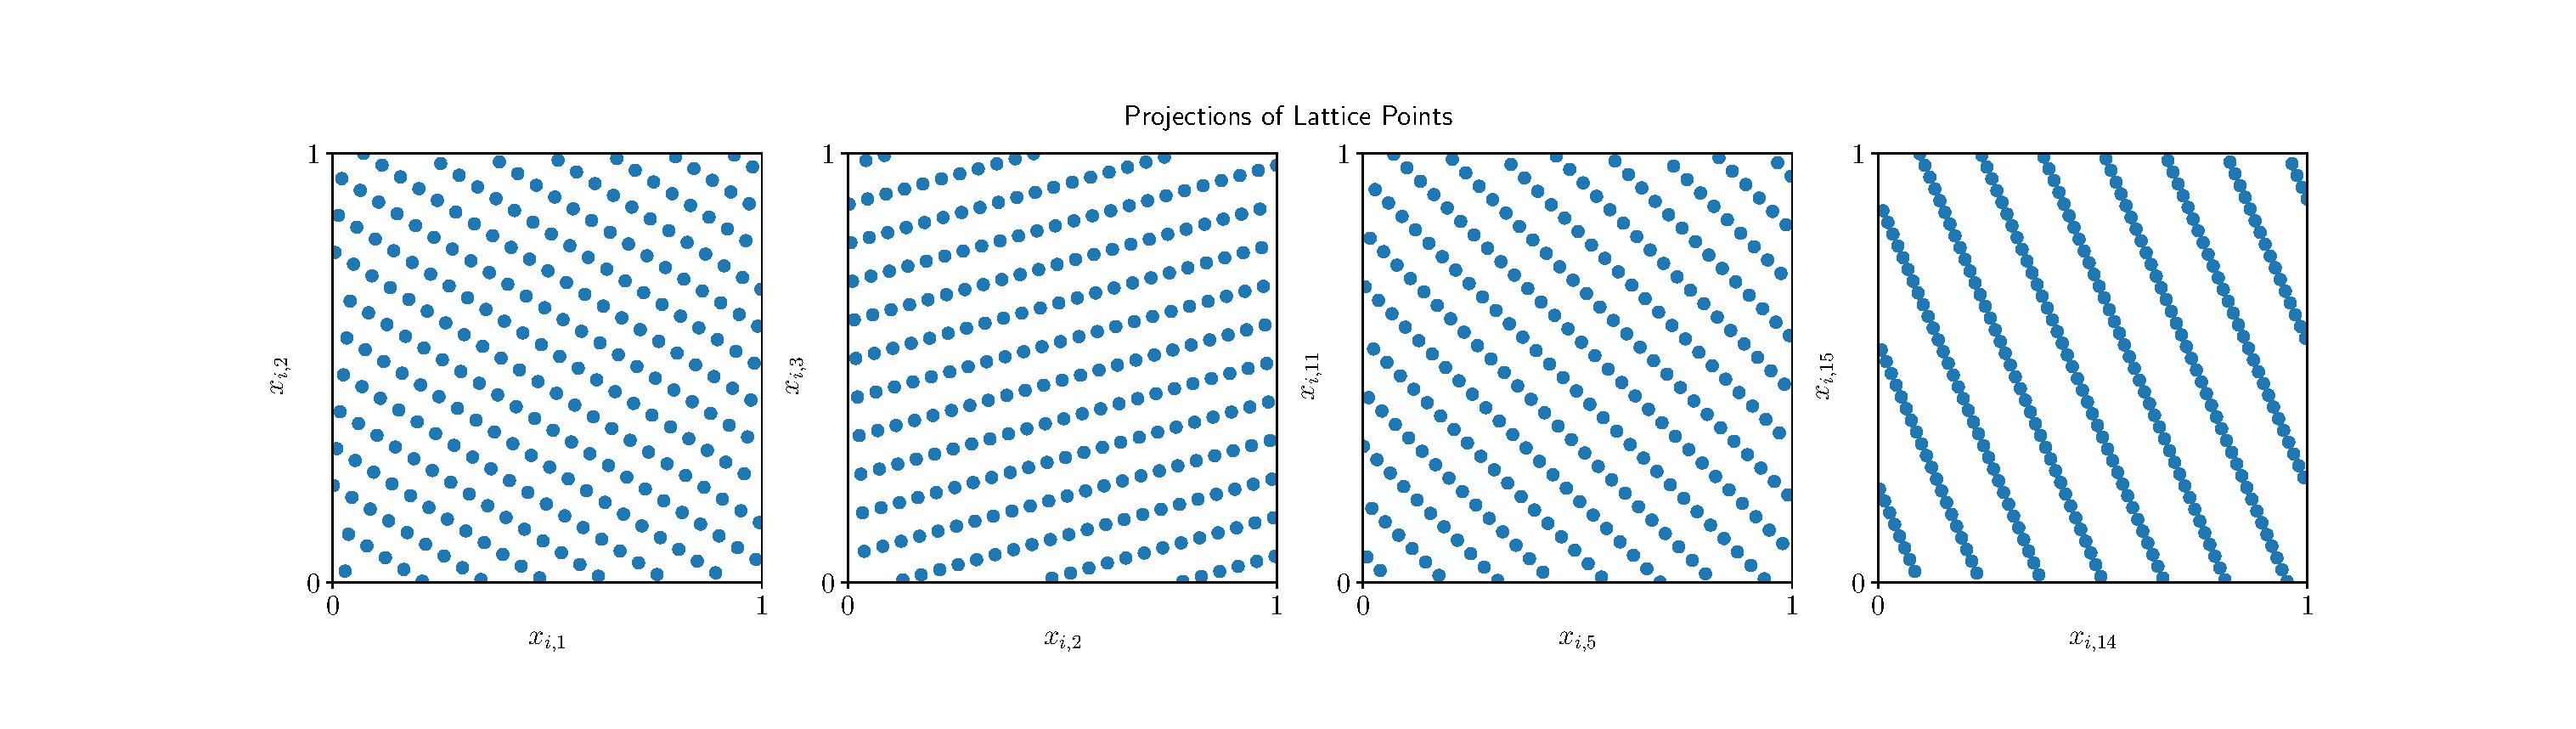
\includegraphics[width=\textwidth]{latticeptsproj.eps}

	\vspace{-4.3ex}

	\includegraphics[width=\textwidth]{sobolptsproj.eps}


\end{frame}

\begin{frame}{Low Discrepancy Points Can Be Randomized}
	\vspace{-3.2ex}

	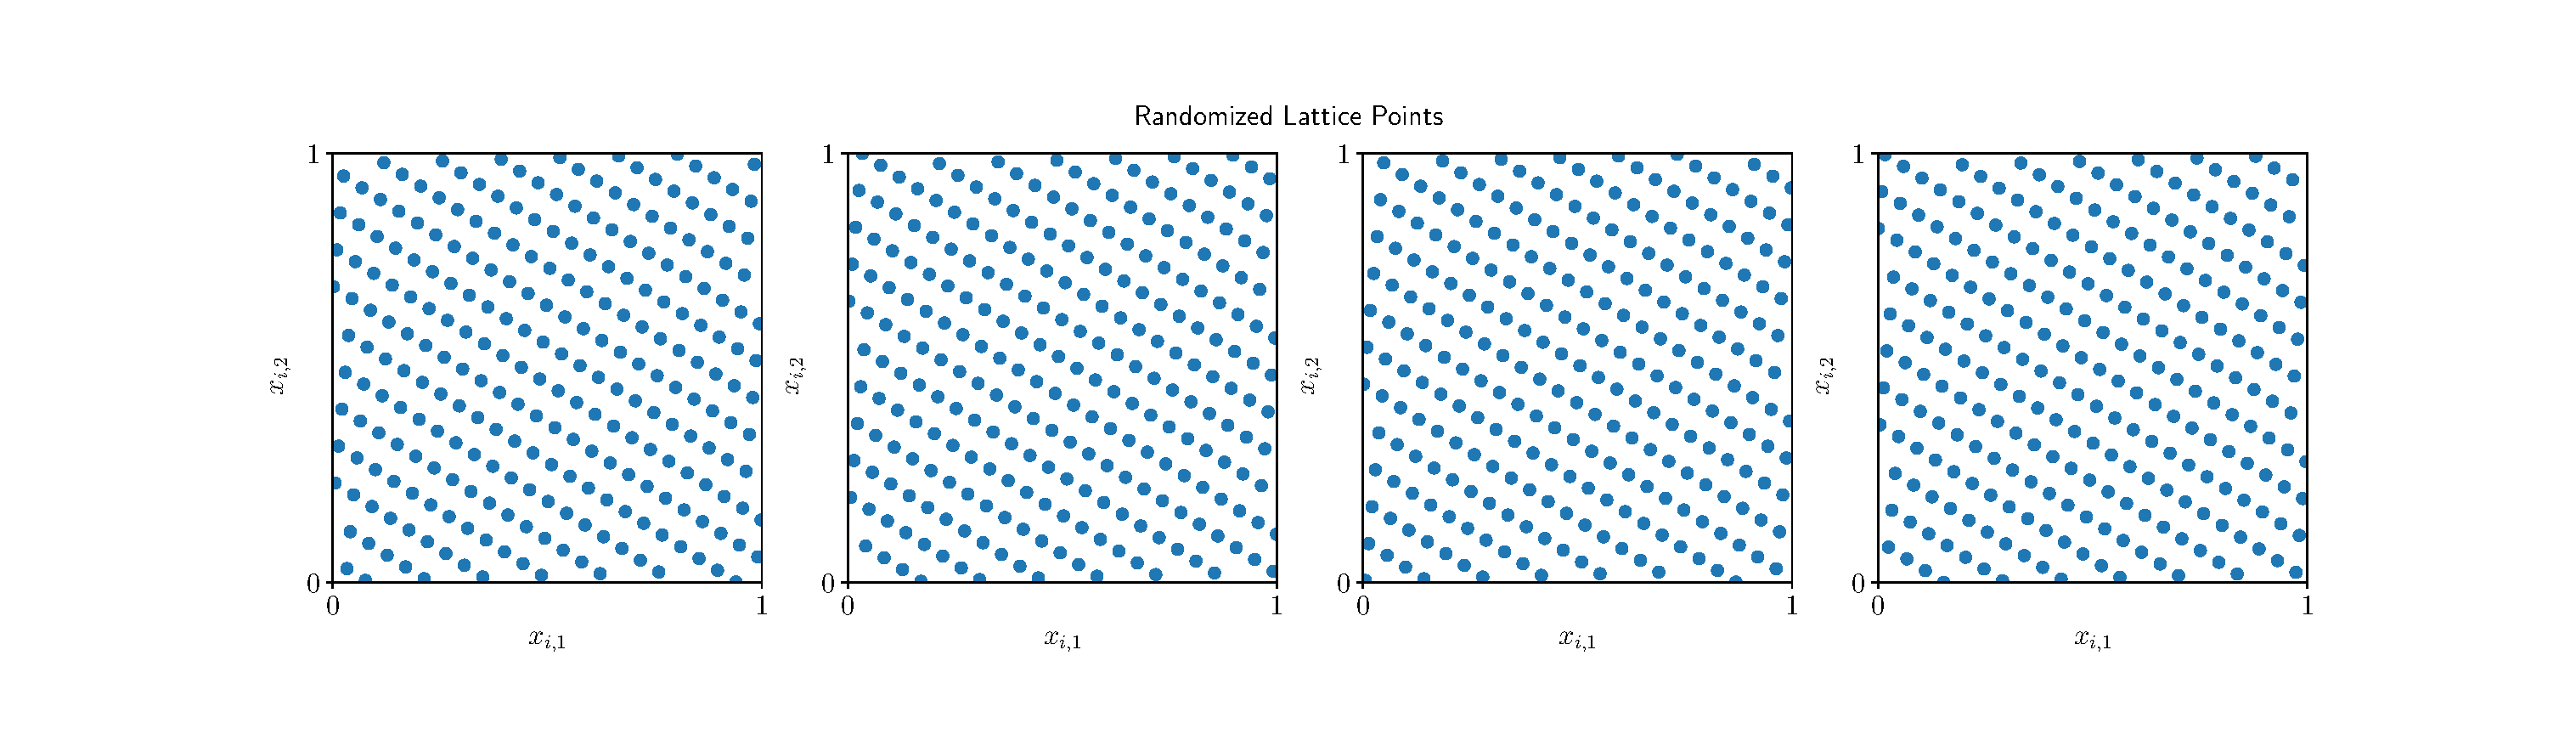
\includegraphics[width=\textwidth]{latticeptsrand.eps}

	\vspace{-4.3ex}

	\includegraphics[width=\textwidth]{sobolptsrand.eps}


\end{frame}

\section{Problems}

\begin{frame}{Research Problems for Consideration}
    \begin{itemize}
        \item Explore quasi-Monte Carlo aka low discrepancy sampling performance using QMCPy on other uncertainty quantification problems in the UM-Bridge suite \footfullcite{umbridge}

        \item Link QMCPy with the finite element solver FEniCSx\footfullcite{LoggEtal_11_2012}

        \item Implement quasi-Monte Carlo Gaussian random fields in 

        \item \{Sou-Cheng insert your problems here\}
        
    \end{itemize}
\end{frame}


\section{Next Steps}

\begin{frame}{If You Want to Dip Your Toes in a Bit More}
    
\end{frame}


\begin{frame}[allowframebreaks]{References}
	\printbibliography
\end{frame}

\end{document}

